\chapter{Introduction}\label{ch:intro}

\section{Background}\label{sec:intro:background}

In today's fast-moving world of technology, data is king.
The ability to quickly and flexibly process large, heterogeneous and asynchronous streams of data, is core to many businesses, and this need is only increasing \cite{Yin_2015}\cite{mit_bean_variety}.

Of particular interest are datasets which are inherently unordered and unbounded.
For instance, consider the issue of tracking listen counts of songs on a service like Spotify, where some views may actually occur on cached data stored offline, and may not be sent to the servers until hours later.
Even more trivially, when operating at a global scale, simple issues like clock skew and network latency mean that we cannot expect data to arrive in-order.

Now, suppose we actually need to aggregate the track listen events into user sessions, defined as listen events occurring sufficiently close to each other.
The amount of complexity and number of special cases even in this reasonable scenario are too large to consider its implementation with dedicated logic.
There is a clear need for an underlying data model and abstraction in order to sanely manage this kind of processing.

Solutions to this problem have been proposed and implemented in open-source systems such as Apache Storm \cite{apache_storm} and Spark Streaming \cite{spark:zaharia2013discretized}, as well as internally in projects like Google's MillWheel \cite{akidau2013millwheel}.
These projects focus on the concept of \emph{stream processing}---the assumption that the inputs are (possibly unbounded, or never-ending) streams of data.
They apply techniques such as windowing, triggering and watermark tracking to make processing this kind of data possible, but in general fall short on sundry features like scalability and fault tolerance, correctness, expressiveness, richness of windowing features, and others.
The key insight is being that these solutions are narrowly scoped for particular problem domains, instead of taking a general approach.

\section{Motivation for the Dataflow Model}\label{sec:intro:motivation}

The issues set out in the previous section drove the development of a new, unified model of data processing at Google.
The seminal paper introducing this model is available~\cite{Akidau:2015} and the reader is invited to refer to it for a full exposition on the development of the model, along with historical and business considerations specific to Google.
This section simply aims to set out the core motivation behind the model, answering the question, ``Why do we need yet another core tool?''

\begin{figure*}[h]
	\centering
	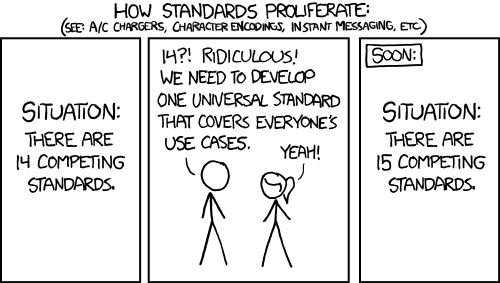
\includegraphics[width=.75\textwidth]{images/xkcd-standards}
	\caption*{\textit{Source: https://xkcd.com/927/}}
\end{figure*}

Simply put, the Dataflow Model aims to provide a unified way of thinking about data processing, producing a clear, composable abstraction.
It acknowledges the fact that it is impossible to design a perfect (always correct, low-latency and cheap) system, and instead it allows for tunability across these characteristics.

\Cref{sec:prep:dataflow} dives deep into the model itself and explains how these aims are achieved, while \cref{ch:impl} contains a detailed overview of the implementation of the model in practice.

\section{Why Elixir?}\label{sec:intro:elixir}

The Elixir language \cite{Elixir} is relatively young (with v1.0 released less than three years ago).
A brief survey of its popular applications reveals that it is most popular in the web development circles, with many treating it as a Ruby replacement.
How then is this a suitable language in which to implement a robust, complex data processing system?

The answer lies in the underpinnings of the language.
Beneath the shiny, modern exterior lies the battle-hardened BEAM VM and OTP framework, which have been running Erlang-powered systems, mostly in the telecommunications industry, for decades.
We also have at our disposal the entire ecosystem of libraries written for Erlang.

\Cref{sec:prep:elixir} gives a more thorough introduction to Elixir, but notable is the fact that it is a dynamically typed, functional language with no variable mutability and with built-in support for efficiently managing and scheduling hundreds of thousands of \emph{processes} (akin to greenthreads) in a manner which is similar to the Calculus of Sequential Processes.
This invites the use of an actor-based model for applications, and indeed this is the standard approach in the Elixir/BEAM ecosystem.
These built-in primitives allow us to closely implement the desired semantics of the Dataflow Model without the overhead of thousands of lines of scheduling, threading and co\"ordinating\footnotemark[1] code (present in the existing Java implementation).

\footnotetext[1]{
For the typographically observant reader: the \"{} mark in ``co\"ordinating'' is a diaeresis---one of the two diacritical marks actually part of English natively (the other being the grave, as in ``the learn\`ed scholar'').
While its use is uncommon in modern English, some publications (notably The New Yorker) still employ it, and including it is the preferred style of the author.
It is used to indicate that two vowels should be pronounced separately, and not as a diphthong.
}

\section{Previous work}\label{sec:intro:previous}
Since the publication of the Dataflow paper \cite{Akidau:2015}, work has been ongoing to implement the Model in practice.
Initially, Google released the Google Cloud Dataflow product \cite{CloudDataflow} along with an SDK to allow users to easily construct data processing pipelines and run them on Google's cloud infrastructure.

In early 2016, Google decided to open-source the project and place it under the care of the Apache Foundation \cite{ApacheDataflowPost}.
This marked the beginning of Apache Beam, a project whose goals were even wider.

One of its main aims was to realise the goal of allowing multiple interchangeable runners to be used from the same SDK, as well as supporting the existence of various compatible SDKs written in different languages.
Each such ``runner'' would be able to take the pipelines created with the SDK and execute them using its own backend, in a way which allows the user to be agnostic of the backend infrastructure.

The project has made excellent progress on these fronts, with a fully-featured SDK written in Java (used as the reference implementation for this project) as well as an actively-developed Python SDK.
There are also various runners for a multitude of data-processing products such as Apache Spark, Apache Storm, Apache Flink and others.
Google Cloud Dataflow remains a paid product capable of running Apache Beam pipelines at scale, but is now only one of many options for doing so.

There is also an on-machine local runner provided in the project, whose main aim is to test workflows on developer machines before running them in the cloud.
As the simplest, yet fully-featured implementation of a Beam runner, it was used as the reference implementation for this project.

Several of the concepts introduced in the Dataflow paper have been used in other project.
Notably, in the Elixir ecosystem, the Flow project \cite{ElixirFlow} takes some of the concepts---such as the windowing and triggering model---and provides a highly idiomatic way to write and execute multi-threaded computation in Elixir.

While the goals and design of Flow are much more narrow than a general Dataflow Model implementation, it itself has driven the development of GenStage \cite{ElixirGenStage}, a more low-level library implementing demand-driven data flow between actor processes, along with an extensible way to route, partition and dispatch that data.
GenStage forms the backbone of the execution logic in this project, and it is described in more detail in \cref{sec:prep:genstage}.

\section{Terminology}\label{sec:intro:terminology}

There are several similar and overlapping terms employed in this document, due to various naming conflicts and naming changes\footnotemark.
This section aims to clarify these and set a convention to be followed in this document.
For a full list of defined terms, the reader should consult the <ref here to Appendix: Glossary>.

\footnotetext[1]{
It seems that even papers and dissertations in Computer Science cannot avoid falling prey to the naming problem.
As is well-known, it is one of the two unsolved problems in the field, the others being cache invalidation and off-by-one errors.
}

Firstly---as noted above---while the original Dataflow Model is due to researchers at Google, and its first implementation was the Google Cloud Dataflow SDK, the project has since been open-sourced and transferred to the Apache Foundation, where it has been renamed Apache Beam.
On the web, the reader will therefore find various references to both the ``Dataflow Model`` and ``Beam Model``, as well as to the implementations themselves, with little consistency.

The approach taken in this paper is to refer to the theoretical model described in \cite{Akidau:2015} as the Dataflow Model, and to the current, de facto official, implementation \cite{ApacheBeam} as Beam (generally referred to in full as Apache Beam).

Further, the virtual machine which powers Erlang and Elixir is called the BEAM.
While efforts are made to refer to the conflicting software in full as the BEAM VM and Apache Beam, the reader should note that wherever the virtual machine is being referred to, BEAM appears in all-uppercase form.

